\documentclass[conference]{IEEEtran}
\IEEEoverridecommandlockouts
\usepackage{cite}
\usepackage{amsmath,amssymb,amsfonts}
\usepackage{algorithmic}
\usepackage{graphicx}
\usepackage{textcomp}
\usepackage{xcolor}
\usepackage{url}
\usepackage{tikz}
\usetikzlibrary{arrows.meta, positioning, calc, fit}
\def\BibTeX{{\rm B\kern-.05em{\sc i\kern-.025em b}\kern-.08em
    T\kern-.1667em\lower.7ex\hbox{E}\kern-.125emX}}
\begin{document}

\title{Performance Comparison of Proof of Authority and Proof of Stake Consensus Mechanisms on DChain National Blockchain Network}

\author{\IEEEauthorblockN{Maulana Anjari Anggorokasih}
\IEEEauthorblockA{\textit{Department of Electrical and Information Engineering} \\
\textit{Faculty of Engineering, Universitas Gadjah Mada}\\
Yogyakarta, Indonesia \\
maulana.anjari2903@mail.ugm.ac.id}
\and
\IEEEauthorblockN{Noor Akhmad Setiawan}
\IEEEauthorblockA{\textit{Department of Electrical and Information Engineering} \\
\textit{Faculty of Engineering, Universitas Gadjah Mada}\\
Yogyakarta, Indonesia \\
noorwewe@ugm.ac.id}
\and
\IEEEauthorblockN{Teguh Bharata Adji}
\IEEEauthorblockA{\textit{Department of Electrical and Information Engineering} \\
\textit{Faculty of Engineering, Universitas Gadjah Mada}\\
Yogyakarta, Indonesia \\
adji@ugm.ac.id}
}

\maketitle

\begin{abstract}
This research evaluates and compares the performance of Proof of Authority (PoA) and Proof of Stake (PoS) consensus mechanisms within DChain, Indonesia's national blockchain infrastructure for higher education electronic certificates. The study is motivated by DChain's planned migration from PoA to PoS to enhance network decentralization and scalability. We employed a quantitative experimental approach through computerized benchmarking using Hyperledger Caliper in a distributed multi-node environment (Docker and Kubernetes). Testing was conducted across various scenarios including throughput, latency, computational resource efficiency, and network stability (soak test). Results indicate that Proof of Stake possesses higher throughput capacity ($\approx$60 TPS) compared to PoA ($\approx$30--40 TPS). However, PoA proved superior in responsiveness, with average latency of 4.6 seconds compared to 8 seconds for PoS, and demonstrated better CPU utilization efficiency. We conclude that the PoA consensus mechanism remains the most optimal solution for DChain's current requirements due to the user-interactive nature of academic services that necessitate rapid response, while PoS offers scalability potential for long-term development.
\end{abstract}

\begin{IEEEkeywords}
Blockchain, DChain, Proof of Authority, Proof of Stake, Benchmarking
\end{IEEEkeywords}

\section{Introduction}

Blockchain technology, first introduced through Bitcoin in 2009, has evolved significantly beyond cryptocurrency applications. The introduction of Ethereum in 2015 with smart contract capabilities expanded blockchain's potential into various sectors. This evolution has driven extensive research into alternative consensus mechanisms more efficient than Proof of Work (PoW), particularly Proof of Authority (PoA) and Proof of Stake (PoS).

In Indonesia, DChain (Dikti Chain) represents a national blockchain network designed to support the higher education ecosystem. DChain functions as a decentralized digital infrastructure enabling the issuance, storage, and verification of academic documents---such as digital diplomas, competency certificates, and transcripts---with guaranteed data integrity. A crucial component determining DChain's performance is the consensus mechanism used to validate transactions and maintain network integrity.

Currently, DChain implements PoA consensus, known for its efficiency as only authorized nodes can validate transactions. However, increasing scale and network complexity necessitate a more decentralized and scalable mechanism like PoS, which allows all token holders to participate in the validation process. This issue aligns with global trends, where Ethereum, one of the largest public blockchains, migrated from PoW to PoS in 2022.

The planned migration from PoA to PoS in DChain raises strategic questions regarding its impact on network performance. To date, no comprehensive study has evaluated consensus migration on DChain using standardized testing parameters. Therefore, this research is designed to analyze and compare DChain's performance under both consensus mechanisms, focusing on metrics such as Transactions Per Second (TPS), latency, computational resource usage, scalability, and system stability.

This research is important to fill this gap by providing empirical foundations for policymakers and developers in determining optimal consensus strategies to support digital transformation in Indonesian higher education.

\section{Related Work}

Several studies have examined the performance of PoA and PoS in blockchain contexts. Choi and Hong \cite{choi2020}, Rebello et al. \cite{rebello2020}, and Arslan et al. \cite{arslan2020} compared both consensus mechanisms based on basic metrics such as Transactions Per Second (TPS) and latency. Their research showed that PoA has advantages in low latency and high throughput under moderate loads, while PoS excels in decentralization and performance at large transaction scales. However, testing was limited to basic performance parameters without analysis of resource usage and system stability.

From a methodological perspective, Li \cite{li2021}, Kumar et al. \cite{kumar2020}, and Kaushal \& Kumar \cite{kaushal2020} emphasized the importance of using benchmarking tools like Hyperledger Caliper for blockchain performance evaluation. This tool enables measurement of standard metrics such as TPS, latency, and resource consumption. Nevertheless, most research only tested one consensus mechanism at a time, thus not providing a comprehensive direct comparison between PoA and PoS.

Scalability and resource efficiency aspects have also been addressed in previous research. Sharma et al. \cite{sharma2020} and Ali et al. \cite{ali2020} found that PoA tends to be more CPU and memory efficient for low to medium loads, while PoS is more stable when facing transaction load variations. However, these studies were generally based on simulations on private Ethereum networks and were not related to the education sector context.

In the educational context, Gaikwad \& Patel \cite{gaikwad2019} and Singh \& Chatterjee \cite{singh2019} emphasized blockchain's role in digital diploma verification and academic data management. Implementations in these studies predominantly used PoA due to its efficiency, but did not examine the potential use of PoS more deeply.

The research most closely approaching this study's focus is by Wicaksono, Hatta, and Aristyagama (2025) \cite{wicaksono2025}. They compared PoA (Ethereum 1.0) and PoS (Ethereum 2.0) on blockchain-based academic transcript systems. Testing was conducted with Hyperledger Caliper using throughput and latency metrics. Results showed that PoA was superior under low to medium loads, while PoS was more suitable for large-scale transactions. However, this research had important limitations: (1) only using two metrics (TPS and latency) without covering resource usage; (2) experiments conducted with one worker in Caliper thus not reflecting multi-user conditions; (3) focus limited to one application (academic transcripts); and (4) no system stability analysis including fault tolerance and fork rate.

This research fills these gaps by expanding testing scope to include resource usage metrics, scalability, and system stability. Additionally, this research applies more diverse benchmarking parameter variations, including number of nodes, block time, block size, transaction load level, transaction operation types, and number of workers. Research focus is directed at DChain as a national blockchain infrastructure for higher education.

\section{Proposed System and Methodology}

\subsection{Experimental Setup}

The research infrastructure consists of:
\begin{itemize}
    \item 1× Control Plane VPS (AMD EPYC, 8 vCPU, 24GB RAM, 200GB NVMe) hosting Caliper orchestrator, Prometheus, Grafana, and PostgreSQL
    \item 5× Worker VPS (heterogeneous: 2× AMD EPYC, 3× Intel Broadwell, 6 vCPU, 12GB RAM, 200GB SSD each) functioning as worker nodes running PoA and PoS consensus protocols
\end{itemize}

Software stack includes:
\begin{itemize}
    \item PoA: Go-Ethereum v1.13.15 + Clique consensus
    \item PoS: Go-Ethereum v1.16.7 + Prysm v6.0.4 (Gasper consensus: LMD-GHOST + Casper FFG)
    \item Benchmarking: Hyperledger Caliper v0.6.0
    \item Monitoring: Prometheus + Grafana + Node Exporter
    \item Orchestration: Kubernetes (k3s) + Kurtosis (for PoS deployment)
\end{itemize}

\subsection{Network Topology}

The experimental topology employs a 10-node configuration consisting of:
\begin{itemize}
    \item \textbf{Control Plane}: Orchestrator sending transaction load (RPC Load) to observer nodes using Hyperledger Caliper
    \item \textbf{Validator Nodes (Signers/Proposers)}: 5 main nodes (V1--V5) with rights to validate transactions and compose new blocks. In PoA consensus, these nodes connect in ring topology for Round-Robin proposer rotation; in PoS, selection is random
    \item \textbf{Observer Nodes (Non-Validators)}: 5 additional nodes (O1--O5) that do not produce blocks but participate in data synchronization through gossip protocol (P2P). These nodes simulate consortium member institutions holding ledger copies without validation rights, functioning as gateways for transactions sent by Control Plane
\end{itemize}

\begin{figure}[htbp]
    \centering
    \resizebox{0.75\columnwidth}{!}{
    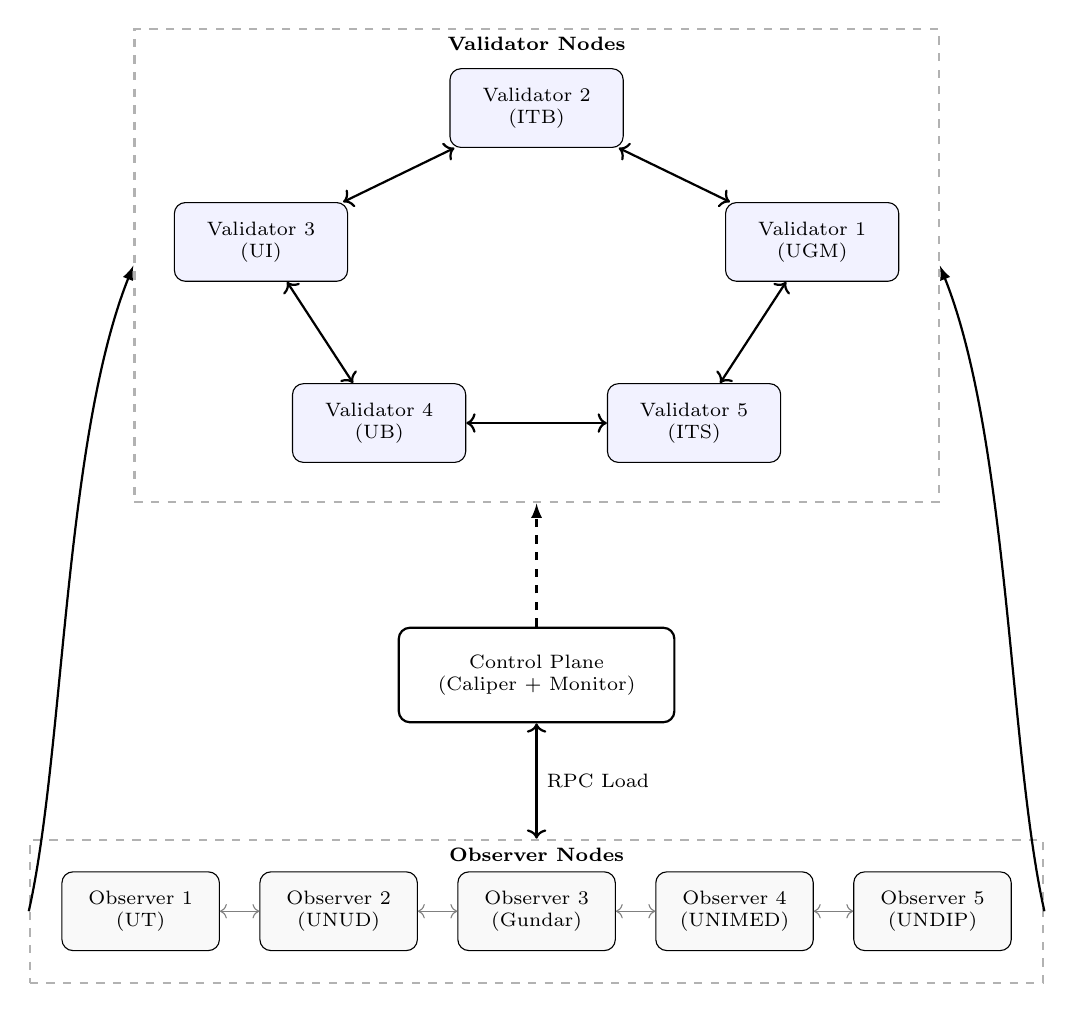
\begin{tikzpicture}[
        node distance=1.5cm,
        validator/.style={rectangle, draw, rounded corners, fill=blue!5, minimum width=2.2cm, minimum height=1cm, align=center, font=\scriptsize},
        observer/.style={rectangle, draw, rounded corners, fill=gray!5, minimum width=2cm, minimum height=1cm, align=center, font=\scriptsize},
        cp/.style={rectangle, draw, rounded corners, thick, fill=white, minimum width=3.5cm, minimum height=1.2cm, align=center, font=\scriptsize},
        groupbox/.style={draw, dashed, thick, inner sep=0.5cm, gray!60},
        arrow/.style={-latex, thick},
        line/.style={draw, -latex, thick}
    ]

        % --- Bottom: Observer Nodes ---
        \node[observer] (O3) at (0, 0) {Observer 3\\(Gundar)};
        \node[observer] (O2) [left=0.5cm of O3] {Observer 2\\(UNUD)};
        \node[observer] (O1) [left=0.5cm of O2] {Observer 1\\(UT)};
        \node[observer] (O4) [right=0.5cm of O3] {Observer 4\\(UNIMED)};
        \node[observer] (O5) [right=0.5cm of O4] {Observer 5\\(UNDIP)};

        % Observer P2P Connections (Gossip)
        \draw[<->, gray, thin] (O1) -- (O2);
        \draw[<->, gray, thin] (O2) -- (O3);
        \draw[<->, gray, thin] (O3) -- (O4);
        \draw[<->, gray, thin] (O4) -- (O5);

        % Observer Group Box
        \node[draw, dashed, thick, gray!60, fit=(O1) (O5), inner sep=0.4cm] (obs_group) {};
        \node[anchor=north, font=\scriptsize\bfseries] at (obs_group.north) {Observer Nodes};

        % --- Middle: Control Plane ---
        \node[cp] (CP) at (0, 3) {Control Plane\\(Caliper + Monitor)};

        % --- Top: Validator Nodes ---
        \begin{scope}[yshift=8cm]
            \node[validator] (V2) at (0, 2.2) {Validator 2\\(ITB)};
            \node[validator] (V1) at (3.5, 0.5) {Validator 1\\(UGM)};
            \node[validator] (V3) at (-3.5, 0.5) {Validator 3\\(UI)};
            \node[validator] (V5) at (2, -1.8) {Validator 5\\(ITS)};
            \node[validator] (V4) at (-2, -1.8) {Validator 4\\(UB)};

            % Validator Bidirectional Ring
            \draw[<->, thick] (V1) -- (V2);
            \draw[<->, thick] (V2) -- (V3);
            \draw[<->, thick] (V3) -- (V4);
            \draw[<->, thick] (V4) -- (V5);
            \draw[<->, thick] (V5) -- (V1);

            % Validator Group Box
            \node[draw, dashed, thick, gray!60, fit=(V1) (V2) (V3) (V4) (V5), inner sep=0.5cm, minimum height=5.5cm] (val_group) {};
            \node[anchor=north, font=\scriptsize\bfseries] at (val_group.north) {Validator Nodes};
        \end{scope}

        % --- Connections ---
        \draw[<->, thick] (CP) -- (obs_group.north) node[midway, right, font=\scriptsize] {RPC Load};
        \draw[arrow] (obs_group.west) .. controls (-6, 2) and (-6, 6) .. (val_group.west);
        \draw[arrow] (obs_group.east) .. controls (6, 2) and (6, 6) .. (val_group.east);
        \draw[dashed, arrow] (CP) -- (val_group.south);

    \end{tikzpicture}
    }
    \caption{Experimental Topology: 10 Nodes with Distributed Infrastructure}
    \label{fig:experimental_topology}
\end{figure}

\subsection{Benchmarking Scenarios}

Five main scenarios were applied to test various performance aspects:

\begin{enumerate}
    \item \textbf{Throughput Capacity (Step Load)}: Find system saturation point (knee point) by gradually increasing TPS load (5, 10, ..., 100 TPS) until latency spikes drastically
    \item \textbf{Fixed Load (Baseline)}: Measure maximum theoretical capacity without send delay by maintaining fixed transaction queue (backlog 20 tx) for 180 seconds
    \item \textbf{Worker Scalability}: Test concurrent client handling efficiency by running optimal TPS load with variations of 1, 3, and 5 workers
    \item \textbf{Read Intensive}: Measure read operation (RPC) performance dominant in real applications with high read loads (200, 400, 600 TPS) on existing data
    \item \textbf{Functional Lifecycle \& Stability}: Test full function (Mint-Read-Burn) and long-term stability through Soak Test for 15 minutes at 60\% optimal load
\end{enumerate}

\subsection{Metrics}

Performance metrics measured include:
\begin{itemize}
    \item \textbf{Transaction Performance}: Throughput (TPS), Latency (avg, P95), Success Rate
    \item \textbf{Resources}: CPU Usage (\%), Memory Usage (MB), Network I/O, Disk I/O
    \item \textbf{Stability}: Stability Index (TPS consistency in long duration)
\end{itemize}

\subsection{Monitoring and Data Collection}

The monitoring system was built using Prometheus collecting metrics from three sources:
\begin{enumerate}
    \item \textbf{Geth/Prysm}: Internal blockchain metrics (peer count, block height, tx pool)
    \item \textbf{Node Exporter/cAdvisor}: Infrastructure metrics (CPU, RAM, Network container)
    \item \textbf{Hyperledger Caliper}: Transaction metrics (TPS, Latency, Errors) sent via Pushgateway
\end{enumerate}
Data was stored in PostgreSQL for further analysis.

\section{Results and Discussion}

\subsection{Throughput and Saturation Point}

Throughput Step testing increased load from 5 to 100 TPS. Results showed that in 10-node topology, PoA began experiencing saturation at load $\approx$30--40 TPS, while PoS maintained linearity up to $\approx$60 TPS before saturation. PoS achieved peak throughput higher than PoA in this configuration.

\begin{figure}[htbp]
    \centering
    \includegraphics[width=0.9\columnwidth]{throughput_curve_zoomed_10_Nodes.png}
    \caption{Throughput Curve on 10-Node Topology}
    \label{fig:throughput_curve}
\end{figure}

\begin{figure}[htbp]
    \centering
    \includegraphics[width=0.9\columnwidth]{optimal_tps_comparison.png}
    \caption{Optimal TPS Comparison}
    \label{fig:optimal_tps}
\end{figure}

\subsection{Transaction Latency}

Latency measurement was conducted under steady-state conditions. The latency trade-off graph shows the relationship between load (TPS) and response time.
\begin{itemize}
    \item \textbf{Baseline Latency}: At low load ($<15$ TPS), PoA has average latency of 4--5 seconds, while PoS ranges 7--8 seconds
    \item \textbf{Latency Under Load}: When approaching saturation point, PoS latency increases sharply compared to PoA which tends to have more stable increases
\end{itemize}

\begin{figure}[htbp]
    \centering
    \includegraphics[width=0.9\columnwidth]{latency_tradeoff_lowload_10_Nodes.png}
    \caption{Latency Trade-off (Hockey Stick Curve) on 10-Node Topology}
    \label{fig:latency_tradeoff}
\end{figure}

\subsection{Resource Efficiency and Scalability}

Efficiency was measured based on TPS ratio per percent CPU usage, and scalability was measured by adding number of client workers. Results showed PoA has much higher CPU efficiency. PoS has significant computational overhead. On client scalability side, both consensuses experienced performance degradation when number of workers increased from 1 to 5, indicating bottleneck on client/RPC side.

\begin{figure}[htbp]
    \centering
    \includegraphics[width=0.9\columnwidth]{efficiency_resource_cpu.png}
    \caption{Resource Efficiency (TPS per \% CPU)}
    \label{fig:efficiency_cpu}
\end{figure}

\subsection{Analysis}

Data shows an interesting phenomenon where PoS actually achieves higher saturation throughput than PoA at 10 Nodes scale. This is suspected to be caused by Block Time limitations. PoA with 5-second blocks has a physical limit on gas amount/block per time unit. Conversely, PoS with 12-second slots, although the interval is longer, allows more efficient transaction batching with the same gas limit per block, producing higher aggregate throughput before RPC saturation.

PoA shows clear superiority in responsiveness aspect. PoA average latency (4.6 seconds) is very close to block time (5 seconds), showing minimal inefficency. Conversely, PoS (8 seconds) suffers from inherent latency from slot mechanism and initial probabilistic finality. For academic service systems, this 3--4 second difference is significant in terms of UX (User Experience).

PoA excels in resource efficiency. PoS "pays" for its decentralization with expensive computation for attestation. Both systems' stability proved robust in long-term testing (Soak Test), with no indication of memory leaks found.

The overall performance profile is summarized in Figure \ref{fig:radar_chart}, showing the trade-off between the two mechanisms across five key dimensions.

\begin{figure}[htbp]
    \centering
    \includegraphics[width=0.8\columnwidth]{radar_chart_comparison.png}
    \caption{Radar Chart Comparison: PoA vs PoS Multidimensional Trade-off}
    \label{fig:radar_chart}
\end{figure}

\subsection{Synthesis: Relevance for DChain}

For academic certificate use cases in DChain, \textbf{PoA} characteristics proved more advantageous because:
\begin{enumerate}
    \item \textbf{User-Interactive}: Low latency provides better user experience
    \item \textbf{Read-Heavy}: Write transaction volume (diploma issuance) is relatively low and seasonal, so PoS massive capacity is less utilized compared to PoA operational cost efficiency
    \item \textbf{Finality}: PoA Clique offers deterministic finality that is simpler for application integration
\end{enumerate}

\subsection{Comparison with Previous Research}

This research provides empirical contribution by comparing DChain testing results with existing literature.

\begin{table}[htbp]
\centering
\caption{Comparison of DChain Results with Previous Literature}
\label{tab:comparison_literature}
\begin{tabular}{|p{1.8cm}|p{2cm}|p{2cm}|p{2cm}|}
\hline
\textbf{Aspect} & \textbf{DChain Findings} & \textbf{Prior Research} & \textbf{Analysis} \\
\hline
Throughput & $\approx$30--40 TPS (Early Saturation) & PoA $>1000$ TPS \cite{choi2020,rebello2020} & DChain results lower due to limited VPS resources and real geographic latency \\
\hline
Latency & $\approx$4--5 seconds & PoA $<1$ second \cite{arslan2020,wicaksono2025} & Consistent with 5-second block time configuration \\
\hline
Efficiency & Very High (TPS/\%CPU) & Considered efficient \cite{sharma2020,ali2020} & Validates finding that PoA is much lighter than PoS \\
\hline
\end{tabular}
\end{table}

This research fills the gap (research gap) with:
\begin{enumerate}
    \item \textbf{Specific Case Study}: Testing functionally relevant workload (Lifecycle), not just token transfer
    \item \textbf{Real Geographic Topology}: Simulation of inter-campus latency (UGM, UI, ITB), not localhost
    \item \textbf{Stability Analysis}: Adding Soak Test to prove system resilience
\end{enumerate}

\section{Conclusion}

This research aimed to evaluate and compare the performance of Proof of Authority (PoA) and Proof of Stake (PoS) consensus mechanisms in the context of implementing higher education electronic certificate infrastructure (DChain). Through comprehensive benchmarking testing using Hyperledger Caliper in a distributed multi-node environment, this research successfully answered the research questions and tested the proposed hypothesis.

Based on empirical data analysis obtained from 300+ test iterations, several main conclusions can be drawn:

\begin{enumerate}
    \item \textbf{Trade-off Between Capacity and Responsiveness}: Results show contradictory performance characteristics between the two algorithms. \textbf{PoS excels in capacity aspect} (throughput) with peak achievement up to $\approx$60 TPS, almost twice as high compared to PoA which experiences saturation at $\approx$30--40 TPS. However, this advantage must be paid with lower responsiveness. \textbf{PoA proved far superior in latency}, recording average confirmation time of 4.6 seconds, significantly faster than PoS ($\approx$8 seconds).
    
    \item \textbf{Resource Efficiency}: In terms of operational efficiency, \textbf{PoA shows superiority} in computational resource utilization. PoA can produce transactions per second per CPU unit (TPS/\%CPU) higher than PoS. This is caused by PoS's more complex architecture, involving two process layers (Execution Layer and Consensus Layer) and intensive gossip communication traffic between validators, thus creating additional computational overhead.
    
    \item \textbf{Suitability with DChain Characteristics}: Considering academic certificate system characteristics that are Read-Heavy (verification dominance compared to issuance), User-Centric (requires fast response during verification), and has moderate transaction volume (seasonal issuance), \textbf{PoA consensus mechanism is deemed more relevant and effective} for implementation in DChain's early consortium stage. Although having lower maximum throughput, 30 TPS capacity is already very adequate to handle daily operational load of higher education institutions, while latency and efficiency advantages provide more crucial added value for user experience and operational costs.
\end{enumerate}

Overall, this research concludes that although PoS offers promises of long-term scalability and wider decentralization, \textbf{PoA remains the most optimal technical solution} for DChain's current needs, balancing performance, cost efficiency, and response speed.

Future research should explore: (1) wider network variables with more nodes ($>20$ nodes) and real WAN geographic conditions; (2) consensus parameter optimization such as reducing block time or increasing block gas limit; (3) security robustness analysis against cyber attack scenarios; and (4) hybrid model studies (PoA-PoS) where PoA serves as sidechain for fast daily operations with periodic checkpointing to main PoS network for long-term security.

\section*{Acknowledgment}

The authors would like to thank the Directorate General of Higher Education, Research, and Technology (Ditjen Diktiristek) for providing access to DChain infrastructure and the participating universities for their support in this research.

All source code, configurations, and datasets used in this research are publicly available at: \url{https://github.com/Skripsi-Maulana-Anjari}

\bibliography{references}{}
\bibliographystyle{IEEEtran}

\end{document}
